\chapter{Literature Review}
\section{Fundamental Equations of Fluid Dynamics}
The basic principle in the study of fluid dynamics is the prediction of fluid motion around objects. To obtain an accurate prediction on fluid's force and momentum around certain objects, mathematical formulation of the physical behaviour of fluid is required. The fundamental equation of fluid dynamics are~\cite{JB}
\begin{enumerate}
\item Continuity equation (conservation of mass)
\item Momentum equation (conservation of linear momentum)
\item Energy equation (conservation of energy)
\end{enumerate}

The philosophy behind above mathematical formulations is based on the assumption that fluid is a continuous medium. 
 
\subsection{Continuity Equation}
Formulation of fundamental equations of fluid dynamics is done by using finite control volume approach. In finite control volume, a closed volume exists within a finite region of the flow. This volume defines a \emph{control volume}, and a \emph{control surface}. The control volume could be fixed with fluid moving through it or moving with the same fluid particles always inside it. Finite control volume model is illustrated in figure~\ref{fig:control_volume}.
\begin{figure}[h]
  \centering
  \scalebox{0.5}{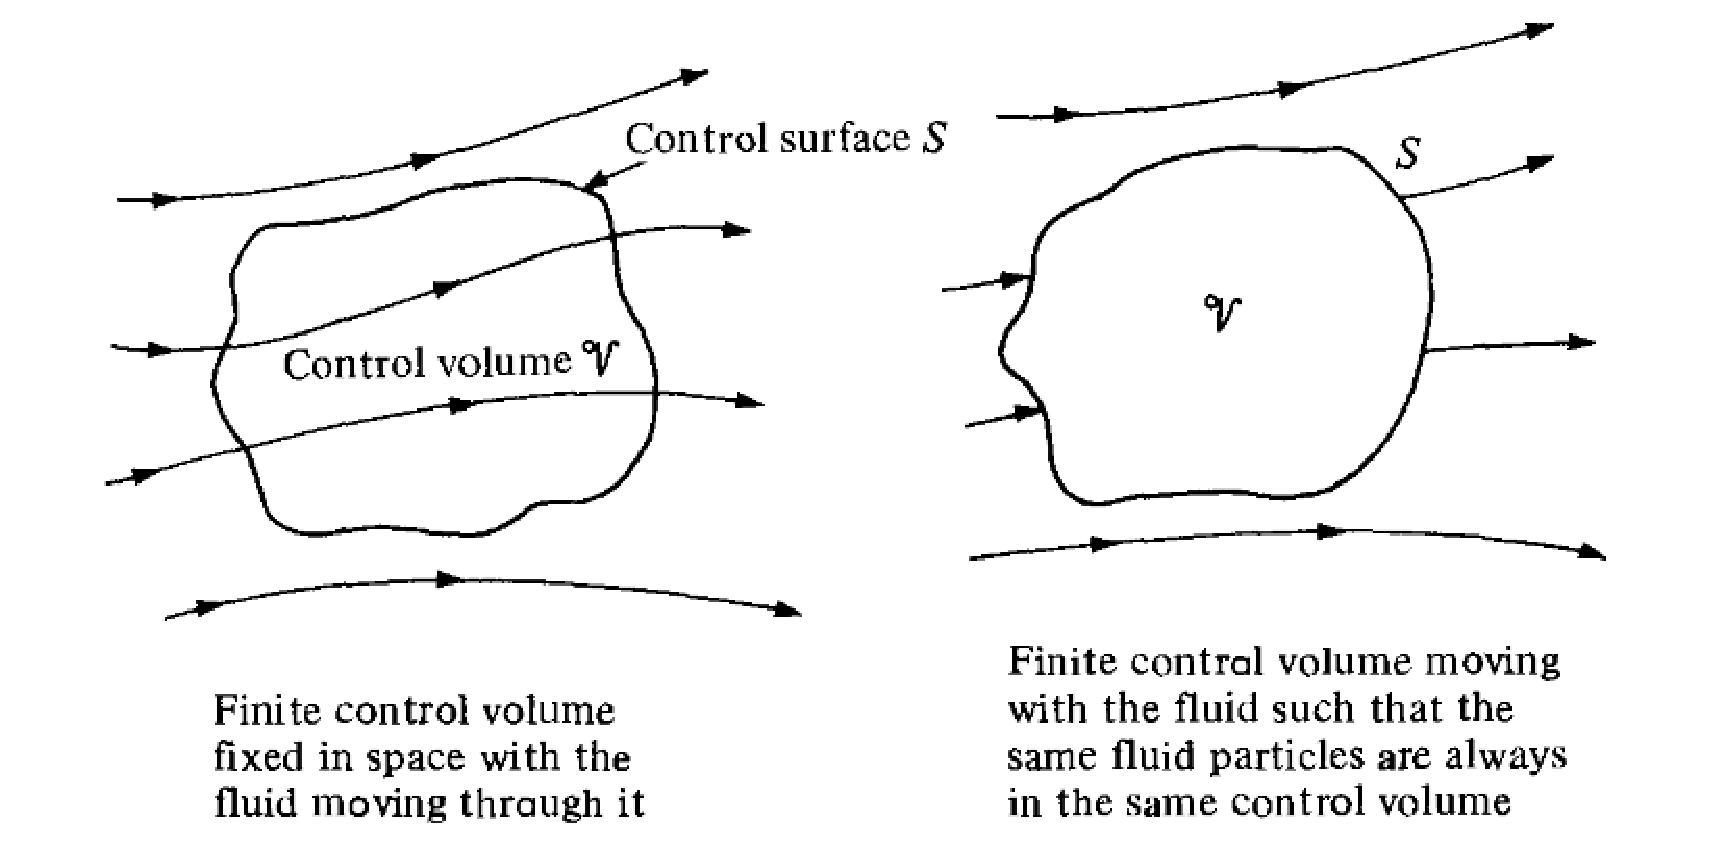
\includegraphics{figures/control_volume.pdf}}
  \caption{Control Volume (\emph{Source:} Reference~\cite{JA})}
  \label{fig:control_volume}
\end{figure}

The physical principle of mass conservation is mass cannot be created or destroyed. When this principle is applied to fixed control volume, it could be interpreted as
\begin{quote}
Net mass flow out of control volume equals time rate decrease of mass inside control volume~\cite{JA}.
\end{quote}  
Based on this assumption, continuity equation can be formulated to equation~\ref{eq:continuity_1}.
\begin{equation}\label{eq:continuity_1}
  \frac{\partial \rho}{\partial t} + \frac{\partial}{x}\left( \rho u \right) + \frac{\partial}{\partial y}\left( \rho v \right) + \frac{\partial}{\partial z}\left( \rho w \right) = 0
\end{equation}
For steady state condition, equation~\ref{eq:continuity_1} can be simplified to equation~\ref{eq:continuity_2}. 
\begin{equation}\label{eq:continuity_2}
\frac{\partial u}{\partial x} + \frac{\partial v}{\partial y} + \frac{\partial w}{\partial z} = 0
\end{equation}

\subsection{Momentum Equation}
Basic physical principle of momentum equation is Newton's second law, which is force equals time rate of change of momentum. When this physical principle is applied to fixed control volume, the momentum equation can be formulated for x direction (equation~\ref{eq:moment_x}).
\begin{equation}\label{eq:moment_x}
\rho\frac{\partial u}{\partial t} + \rho u\frac{\partial u}{\partial x} + \rho v\frac{\partial u}{\partial y} + \rho w\frac{\partial u}{\partial z} = \rho f_x - \frac{\partial p}{\partial x} + \mu\left(\frac{\partial^2u}{\partial x^2} + \frac{\partial^2u}{\partial y^2} + \frac{\partial^2u}{\partial z^2}\right)
\end{equation}
The same formulation can be done for y and z direction.
\begin{equation}\label{eq:moment_y}
  \rho\frac{\partial v}{\partial t} + \rho u\frac{\partial v}{\partial x} + \rho v\frac{\partial v}{\partial y} + \rho w\frac{\partial v}{\partial z} = \rho f_y - \frac{\partial p}{\partial y} + \mu\left(\frac{\partial^2v}{\partial x^2} + \frac{\partial^2v}{\partial y^2} + \frac{\partial^2v}{\partial z^2}\right)
\end{equation}
\begin{equation}\label{eq:moment_z}
   \rho\frac{\partial w}{\partial t} + \rho u\frac{\partial w}{\partial x} + \rho v\frac{\partial w}{\partial y} + \rho w\frac{\partial w}{\partial z} = \rho f_z - \frac{\partial p}{\partial z} + \mu\left(\frac{\partial^2w}{\partial x^2} + \frac{\partial^2w}{\partial y^2} + \frac{\partial^2w}{\partial z^2}\right)
\end{equation}
Equation~\ref{eq:moment_x}, \ref{eq:moment_y}, and~\ref{eq:moment_z} are known as \emph{Navier -- Stokes} equations. These equations are the fundamental equations to predict force and momentum of fluid around objects.

\section{Boundary Layer Theory}
Although Navier -- Stokes equation is regarded as the fundamental equation in fluid dynamics, until today it has no exact solution. This is because Navier -- Stokes is a nonlinear partial differential equation. Fortunately two main fluids, air and water, have a low viscosity which allow simplification on the fundamental equation. However, this does not justify the omission of viscosity term completely. A complete omission will cause the solution of the simplified equation could not satisfy the complete boundary conditions. 

On 1904, Ludwig L. Prandtl published boundary layer theory. This theory simplify the Navier -- Stokes equations by dividing the flow field into two regions based on its distance from the object's surface, which are~\cite{JB}
\begin{itemize}
\item Viscous boundary layer adjacent to object's surface
\item Inviscid flow outside the boundary layer
\end{itemize}
The schematic of boundary layer can be seen in figure~\ref{fig:boundary_layer}
\begin{figure}[h]
  \centering
  \scalebox{0.5}{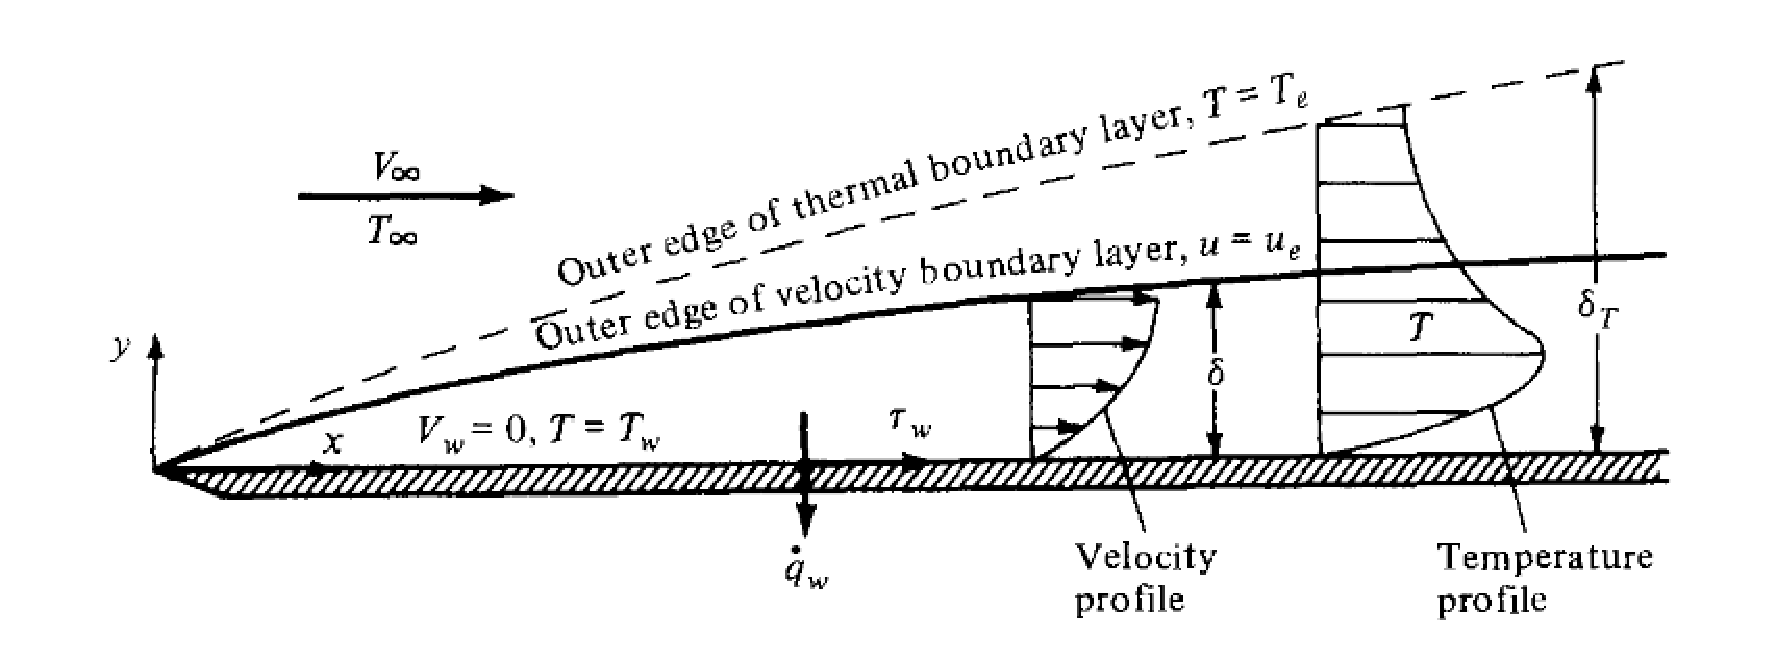
\includegraphics{figures/boundary_layer.pdf}}
  \caption{Schematic of boundary layer (\emph{Source:} Reference~\cite{JA})}
  \label{fig:boundary_layer}
\end{figure}

In boundary layer theory, the momentum equation can be simplified into equation~\ref{eq:boundary_layer}.
\begin{equation}\label{eq:boundary_layer}
  \rho u\frac{\partial u}{\partial x}+\rho v\frac{\partial u}{\partial y} = \rho_eu_e\frac{du_e}{dx}+\nu\frac{\partial^2u}{\partial y^2}
\end{equation}

\subsection{Boundary Layer Properties}
Two frequently used boundary layer properties are \emph{displacement thickness} $(\delta^*)$ and \emph{momentum thickness} $(\theta)$~\cite{JA}. Displacement thickness is illustrated in figure~\ref{fig:displ_thick}. Figure on left shows the ideal streamline flow for inviscid case where boundary layer does not exist in object's surface. In this condition, streamline is parallel to object's surface. In constrast to previous condition is actual streamline flow, which is shown by figure on right where boundary layer exists at object's surface. The presence of boundary layer will cause streamline to shift. The distance in which streamline shifted is called displacement thickness. 
   
\begin{figure}[h]
  \centering
  \scalebox{0.5}{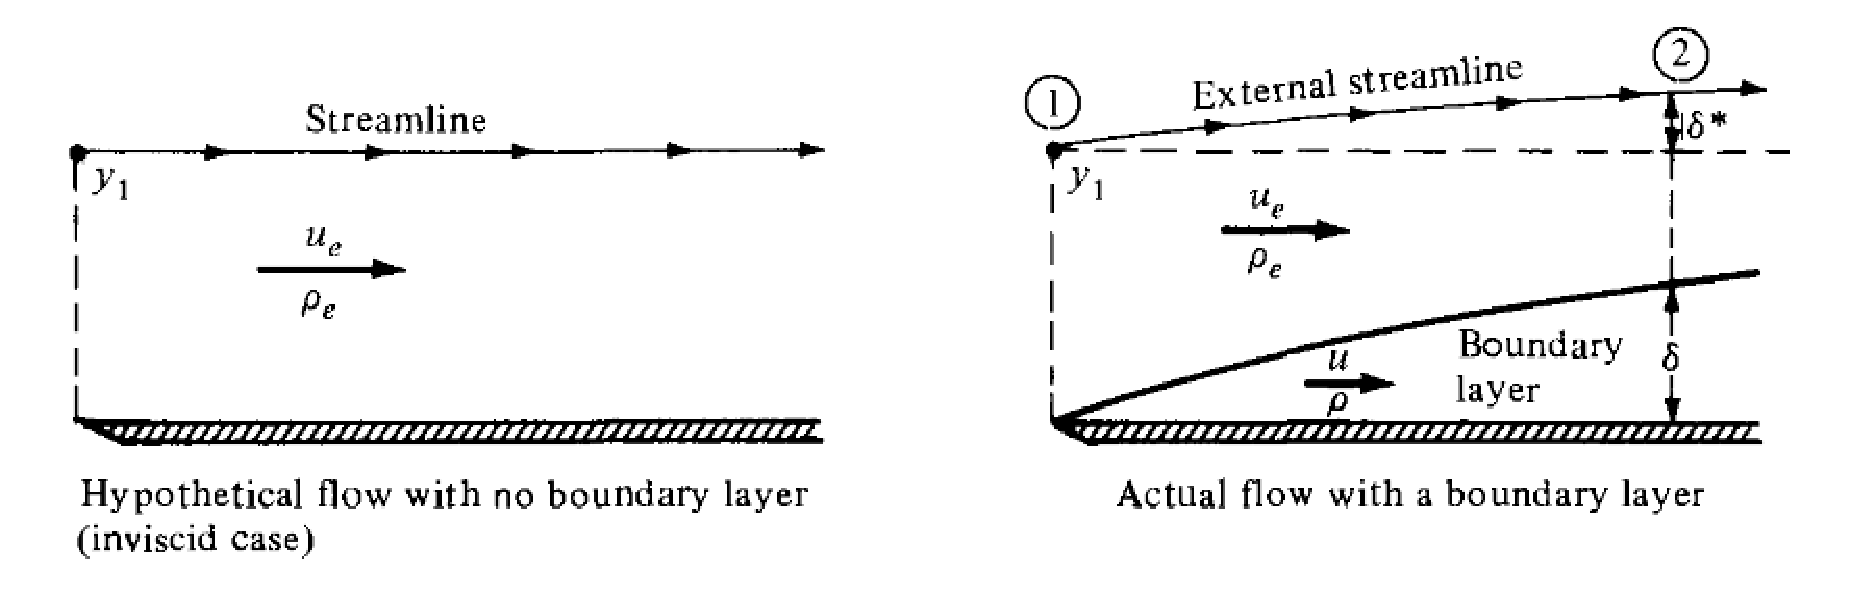
\includegraphics{figures/displ_thick.pdf}}
  \caption{Schematic of displacement thickness (\emph{Source:} Reference~\cite{JA})}
  \label{fig:displ_thick}
\end{figure}

Displacement thickness can also be interpreted as index proportional to the ''missing mass flow'' due to the presence of the boundary layer~\cite{JA}. This interpretation is related to mathematical formulation of displacement thickness as can be seen in equation~\ref{eq:displ_thick}
\begin{equation}\label{eq:displ_thick}
\delta^* = \int_{0}^{\delta} \left(1-\frac{u}{u_e}\right)dy
\end{equation}

The second most important boundary layer properties is momentum thickness. Physical interpretation of momentum thickness is momentum loss due to the presence of boundary layer~\cite{PK}. Mathematical formulation of momentum thickness is shown by equation~\ref{eq:momentum}
\begin{equation}\label{eq:momentum}
\theta = \int_{0}^{\delta} \frac{u}{u_e} \left(1-\frac{u}{u_e} \right) dy
\end{equation}

It should be noted that the concept of momentum thickness is useful in prediction of drag coefficient. The relation between momentum thickness and drag coefficient is shown in equation~\ref{eq:cf}, where $L$ is length.
\begin{equation}\label{eq:cf}
C_f = \frac{2\theta}{L}
\end{equation}

\subsection{Boundary Layer in flat plate (Blasius Solution)} 
One of aerodynamics theory application is airfoil. If an infinitesimal length of airfoil's surface is observed, it can be seen as a flat plate. Heinrich Blasius (1908), a student of Prandtl,  performed application of boundary layer theory on a flat plate for the first time on his PhD thesis. This application is known as \emph{Blasius Solution}, which became one of the basic theory behind many boundary-layer theory.

In Blasius equation, a case of incompressible, two-dimensional flow over a flat plate at $0^o$ angle of attack. From such condition, Navier -- Stokes equation is transformed from partial differential equation to \emph{ordinary differential equation} as shown in equation~\ref{eq:blasius}.
\begin{equation}\label{eq:blasius}
2f''' + f f''=0
\end{equation}
Although the Navier -- Stokes equation is simplified to ordinary differential form, the nature of the equation is still nonlinear, which can only be solved numerically.

When above equation is plotted in graph $f'(\eta)=u/u_e$ as a function of $\eta$ (figure~\ref{fig:vel_profile_1}) it can be seen that $u$ will change when the flow move downstream. However, when plotted in graph versus $\eta$ (figure~\ref{fig:vel_profile_2}), it can be seen that $u = u(\eta)$ profile is the same as the flow progress downstream. This \emph{similarity} is called \emph{self-similarity solution}~\cite{JA}. Self-similar profile can only be found on a certain type of flows. Boundary layer profile for flows over an arbitrary body are \emph{nonsimilar}.
\begin{figure}[h]
  \centering	
  \scalebox{0.5}{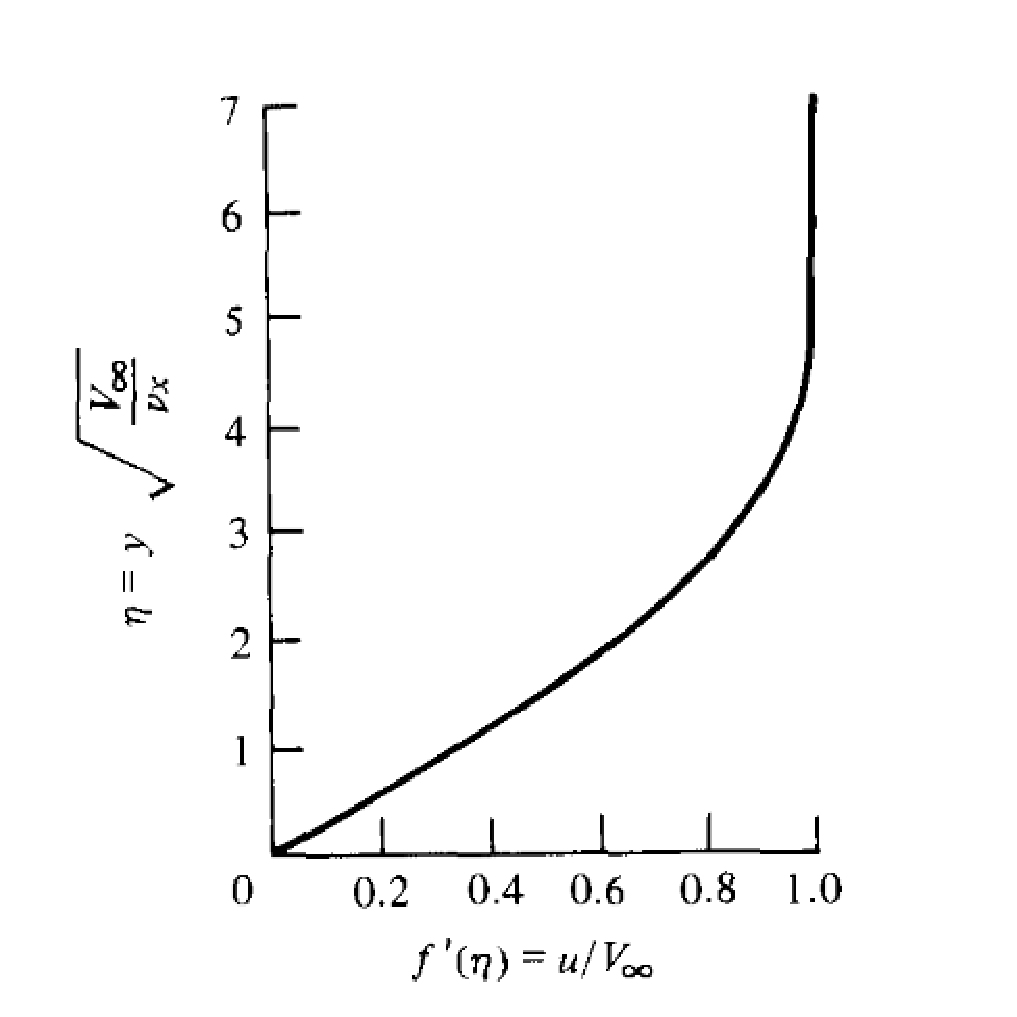
\includegraphics{figures/vel_profile_1.pdf}}
  \caption{Incompressible velocity profile for a flat plate; solution of the Blasius equation.(\emph{Source:} Reference~\cite{JA})}
  \label{fig:vel_profile_1}
\end{figure}

\begin{figure}[h]
  \centering
  \scalebox{0.5}{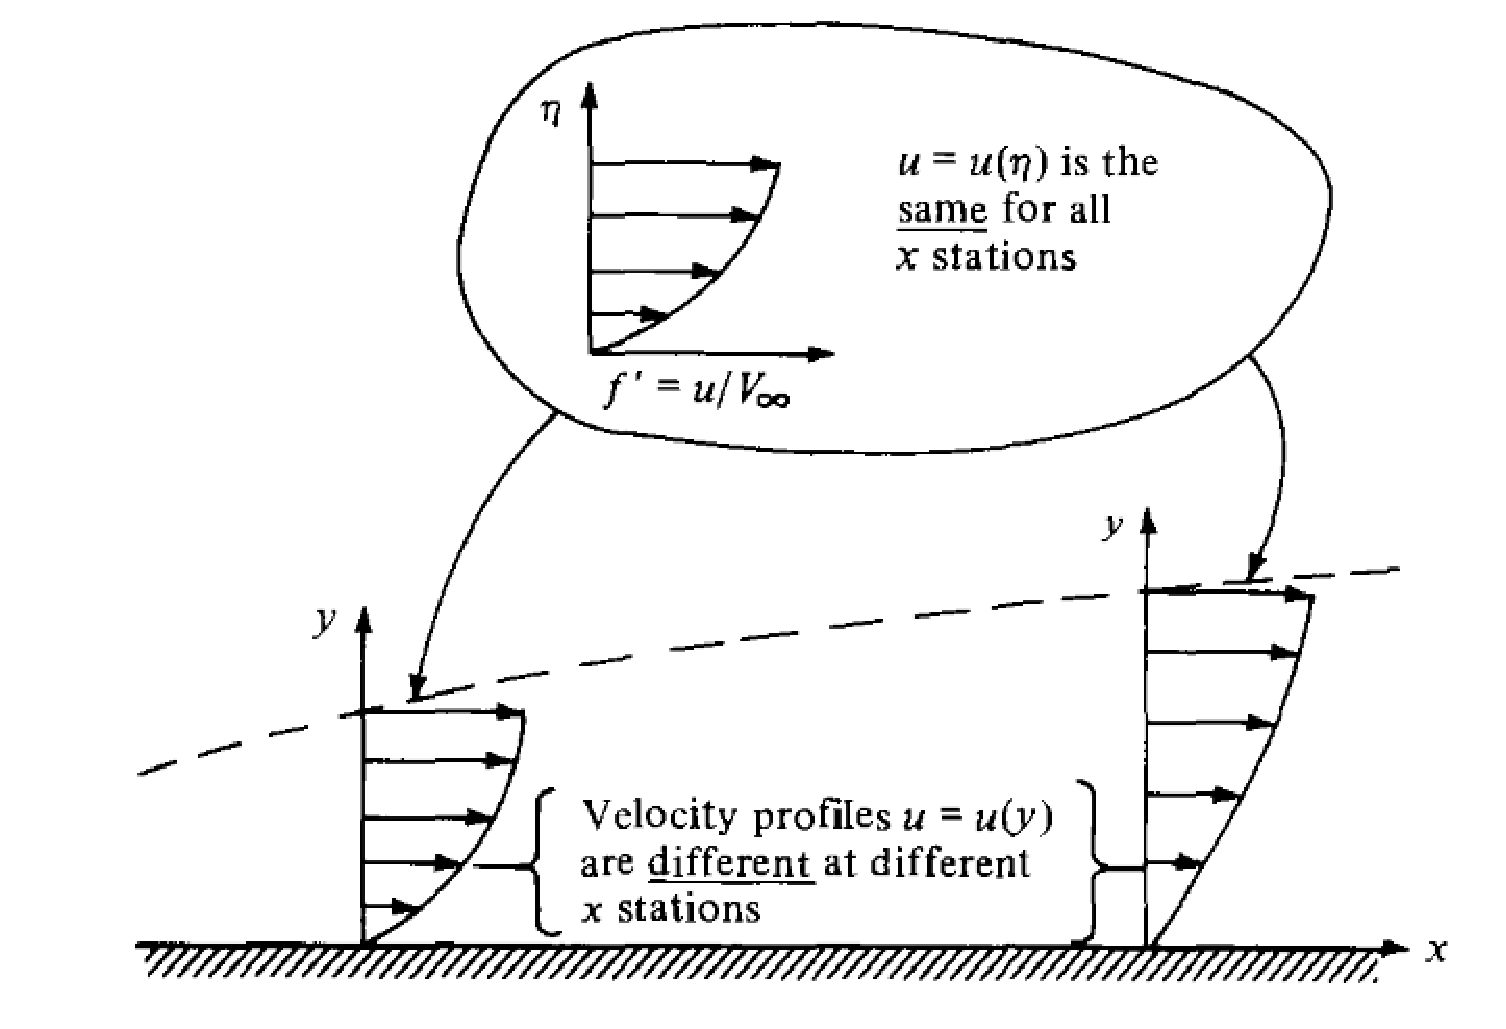
\includegraphics{figures/vel_profile_2.pdf}}
  \caption{Velocity profile in physical and transformed space, demonstrating the meaning of self-similar solution.(\emph{Source:} Reference~\cite{JA})}
  \label{fig:vel_profile_2}
\end{figure}

\subsection{Laminar boundary layer}
Boundary layer could be divided into two areas, \emph{laminar}and \emph{turbulent} boundary layer. In laminar boundary layer area, the momentum transfer in the direction perpendicular to the flow happens in molecular/microscopic scale. Because of molecular movement, \emph{slower-moving} fluid particles from lower layer will move upward and slowing the particles in upper layer. In other side, when upper layer \emph{faster-moving} fluid particles moves downward, it will accelerate the lower layer fluid particles~\cite{JB}. Figure~\ref{fig:comparison} illustrates the phenomena explained before.

\begin{figure}
  \centering
  \scalebox{0.7}{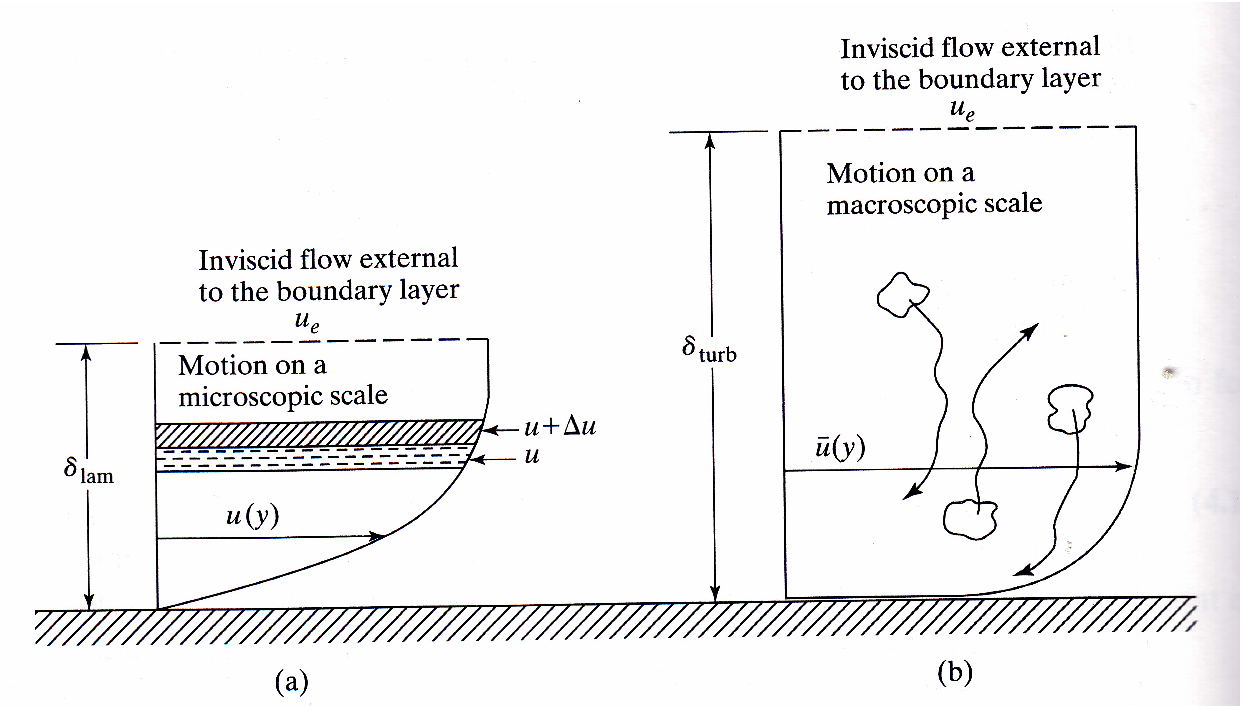
\includegraphics{figures/comparison.pdf}}
  \caption{(a) Laminar, (b) Turbulent}
  \label{fig:comparison}
\end{figure}

The laminar boundary layer properties for Blasius equations can be obtained through numerical calculation of equation~\ref{eq:blasius}. Some of the important properties are skin friction coefficient (equation~\ref{eq:laminar_cf}) and boundary layer thickness (equation~\ref{eq:laminar_blthickness}).

\begin{equation} \label{eq:laminar_cf}
  C_f = \frac{1.328}{\sqrt{Re_c}}
\end{equation}

\begin{equation} \label{eq:laminar_blthickness}
  \delta = \frac{5.0x}{\sqrt{Re_x}}
\end{equation}

\subsection{Turbulent boundary layer}
Transformation of laminar boundary layer to turbulent boundary layer does not takes place instantly. \emph{Transition} area exists between both boundary layers. The length of transition area can be the same as laminar boundary layer length. The physical principle behind the laminar boundary layer transformation to turbulent can be described as follow. The boundary layer formed in object's surface is subjected to numerous disturbance, e.g. surface roughness, temperature irregularities, background noise, etc. For some flow, these disturbances are damped which make boundary layer stay laminar. However, for some other type of flow, the disturbances are amplified and the boundary layer becomes turbulent. 

In constrast with laminar boundary layer, in turbulent boundary layer the momentum transfer takes place in a macroscopic scale. Thus, in addition to laminar shear stress, a large \emph{turbulent shear stress} exist along the same direction.

Due to slower-moving fluid particles near the wall are transported well upward, turbulent boundary layer has a relatively large thickness. Turbulent boundary layer also has larger shear stress than a laminar boundary layer. This is because faster-moving fluid particles are transported toward the wall and produce relatively high velocity for the fluid particles near the surface.

Since turbulent flow is highly unpredictable, turbulent boundary layer properties for flat plate are obtained from empirical data. Some important properties are shown in equation~\ref{eq:turbulent_cf} and~\ref{eq:turbulent_blthickness}

\begin{equation} \label{eq:turbulent_cf}
  C_f = \frac{0.074}{\sqrt{Re_c^{1/5}}}
\end{equation}

\begin{equation} \label{eq:turbulent_blthickness}
  \delta = \frac{0.37x}{\sqrt{Re_x^{1.5}}}
\end{equation}

When the boundary-layer thickness for turbulent boundary layer (equation~\ref{eq:turbulent_blthickness}) is compared with laminar boundary layer (equation~\ref{eq:laminar_blthickness}), it could be seen that turbulent boundary-layer thickness grow more rapidly than its laminar counterpart. In other side, turbulent boundary layer also produces larger wall friction coefficient, as can be seen from the comparison between equation~\ref{eq:turbulent_cf} and~\ref{eq:laminar_cf}.

\section{Computational Fluid Dynamics}
Although boundary layer theory greatly simplify Navier -- Stokes equation, there are still no exact analytical solution for the fundamental equations. The main hurdle is because Navier -- Stokes equation is a nonlinear partial differential equation, which has no exact solution exist until today. 

Computational Fluid Dynamics (CFD) is a study of fluid mechanics that heavily utilize numerical analysis and algorithms to solve and analyze fluid dynamics problems~\cite{Wiki}. In contrast with solution provided by analytical solution, CFD result is a collection of numbers that represents the approximate solution of Navier -- Stokes equation. 

With advancement of computer technology, CFD has gained its popularity in engineering application. Many engineering problems that cannot be done by experiment method, has been solved with CFD methods. Some of the advantages of CFD method are 
\begin{itemize}
\item Less time and financial resources needed in solving problem.
\item CFD methods have solve many problems that previously cannot be done by
experimental methods due to environment constraints etc. 
\end{itemize} 

The basic principle of numerical analysis is to breakdown continuous mathematical function into algebraic equation. This can be done through discretization method, which is one of the important aspect in Computational Fluid Dynamics. There are few discretization methods used in CFD, e.g. \emph{Finite Difference Method}, \emph{Finite Element Method (FEM)}, \emph{Finite Volume Method}, spectral method, etc.

\subsection{Direct Numerical Simulation}  
In fluid dynamics, study of turbulence is considered as one of the interesting subject. Turbulence is largely consist of mixture between order and chaos and possess a wide range of length and time scales~\cite{parviz}. Due to the limitation of past computer technology, it was impossible to solve turbulence problem by using only Navier -- Stokes equation. Hence, turbulence modelling was introduced as a complement, e.g.  RANS (Reynolds-Averaged Navier -- Stokes) and LES (Large Eddy Simulation). Turbulence model can be used to approximate or to average the number of turbulent statistics in the flow. By using turbulence model, turbulent flow computation can be simplified.  However, with the increase of flow complexity, a better computation tool is needed.

\emph{Direct Numerical Simulation (DNS)} is computational fluid dynamics simulation method where Navier -- Stokes equation is solved without turbulence model. Since the computation is done without any simplification, DNS's accuracies are very high. To ensure that the computation able to contain all the significant turbulent statistics, DNS method requires a very large scale of computation.

With regards to its computation scale, DNS method is very time consuming. Even with the state of art computer technology, it is still limited to flow with relatively low Reynolds numbers and geometrically simple domain. Although it provides a very detailed information,  DNS result is deemed superfluous and too expensive for commercial purpose. On the other hand, DNS has gained a lot of attention in academical research and has been applied as research tool to some applications. Some example on which DNS has been applied are~\cite{ferziger}:

\begin{itemize}
\item Understanding the mechanism of turbulence production, energy transfer, and dissipation in turbulent flows
\item Simulation of the production of aerodynamics noise
\item Understanding the effects of compressibility on turbulence
\item Understanding the interaction between combustion and turbulence
\item Controlling and reducing drag on a solid surface
\end{itemize}

For simple geometry, DNS has been done by using spectral method to discretize Navier -- Stokes equation~\cite{chung}. The streamwise and spanwise directions are discretized by using \emph{Fourier series} and wall-normal direction by \emph{Chebysev polynomials} or \emph{B-splines}. However, spectral method applications are only limited to simple geometry. For complex geometries, DNS has been carried out by using finite difference method with less accuracy. In recent years, the application of finite element method and unstructured grid are being explored~\cite{parviz}.

\subsection{Spectral method}
Spectral method are a class of spatial discretizations for differential equations~\cite{canuto}. Spectral method consist of basis functions which will provide approximate solutions. The choice of basis functions in spectral method is the feature that distinguish it from other discretization methods such as finite element method.  Finite element method's basis function acts as \emph{local} functions, which are polynomials with low degree. In contrast with finite element method, spectral method's basis functions acts as \emph{global} functions, which are polynomials with high degree, e.g. Fourier series, Chebysev polynomials, etc~\cite{boyd}. The choice of basis functions provide pro and cons for both methods. Finite element method can be fitted to complex geometries enough flexibility, however it suffers for low accuracy. On the other hand spectral method produce a high accuracy, but its applications are limited only to regular and smooth geometry.

Although spectral method's error converges faster than other discretization methods, e.g. finite difference method, it is not the best method available. The drawbacks of spectral method are:
\begin{itemize}
\item Spectral method's algorithms are more difficult to program
\item More expensive with the increase of degree of freedom 
\item Low performance in complex geometries
\end{itemize}
 
\subsection{Verification and Validation}
Software used in this project is \emph{Simson}. This software is developed in Royal Institute of Technology, Sweden. This software has been used in several research projects, e.g. Skote et al.~\cite{skote-1}, Henkes et al.~\cite{skote-2} and etc. In Skote et al.~\cite{skote-1}, the numerical result on turbulent statistics of zero pressure gradient and adverse pressure gradient show an agreement with the experimental result. In Henkes et al.~\cite{skote-2} a few turbulent models are evaluated. From the few methods, Differential Reynolds Stress Model (DRSM) shows good agreement with experimental results, while algebraic model and $k-\omega$ models show reasonably accurate result. However $k-\epsilon$ model gives a rather large deviations for strong adverse pressure gradients. 